% Independent columns let prose follow the shorter table immediately.
\newpage
\suppressfloats[t]
\noindent\begin{minipage}[t]{\columnwidth}\vspace{0pt}
\centering
\captionsetup{position=top,skip=7pt}
\captionof{table}{\textbf{ECP improves Rope planning.} Fixed DINO-WM, three pushes per plan. Ours adds fixed-strength memory after five warm-up pushes. Twenty targets repeat under three seeds (60 runs). CD is mean final Chamfer distance; success requires CD $<0.3$.}
\label{tab:rope}
\small
\begin{tabular*}{\linewidth}{@{\extracolsep{\fill}}lrrr@{}}
\toprule
Method & CD $\downarrow$ & Success (\%) $\uparrow$ & Pushes $\downarrow$\\
\midrule
DINO-WM (native) &0.6865&55.0&12.68\\
DINO-WM (ours) &\textbf{0.4793}&\textbf{71.7}&\textbf{11.30}\\
\bottomrule
\end{tabular*}
\end{minipage}
\par\vspace{8pt}
\begin{figure}[t]
\centering
\captionsetup{skip=5pt}
\makebox[\columnwidth][c]{\hspace*{-6pt}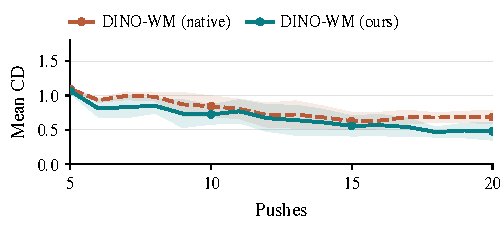
\includegraphics[width=0.92\columnwidth]{figures/fig_rope_cd_pushes.pdf}\hspace*{6pt}}
\caption{\textbf{Faster Rope error reduction.} Mean Chamfer distance (CD; lower is better) versus executed pushes. ECP reduces error faster and reaches a lower final error than native DINO-WM; shaded bands show variability across three seeds.}
\label{fig:rope-cd}
\end{figure}
